\subsection{Основная информация об алгоритме Эрли}

Пусть $w \in \Sigma^*$ — слово на входе. На вход подаётся контекстно-свободная грамматика $G = \langle N, \Sigma, P, S \rangle$.

\Def Ситуация — объект вида $\brackets{A \rightarrow \alpha \cdot \beta, i}$, где правило $\brackets{A \rightarrow \alpha \beta} \in P$, $\cdot$ — вспомогательный символ, который не принадлежит ни $\Sigma$, ни $N$, $i \in [0; |w|]$.

\Def $D_j$ — множество ситуаций вида $\brackets{A \rightarrow \alpha \cdot \beta, i}$ таких, что $\alpha \vdash w[i : j]$.

\Note Вывод считаем левосторонним: пусть правило $\brackets{A \rightarrow \beta} \in P$, тогда:

\begin{center}
    $S \vdash \varphi A \psi \vdash_1 \varphi \beta \psi \Longrightarrow \varphi \in \Sigma^*$
\end{center}

\Note Ситуация $\brackets{A \rightarrow \alpha \cdot \beta, i} \in D_j$ означает, что:

\begin{enumerate}
    \item $S \vdash w [0 : i]$, где $S$ — стартовый нетерминальный символ;
    \item $\brackets{A \rightarrow \alpha \beta} \in P$;
    \item $\alpha \vdash w[i:j]$.
\end{enumerate}

\textit{Если вдруг с алгоритмом Эрли вы встречаетесь впервые, то представьте, что точка играет роль курсора, слева от которого то, что уже было введено, а справа находится то, что предстоит обработать.}

\Note Для удобства вводится новый стартовый нетерминальный символ $S'$, а также в грамматику $G$ добавляется правило $\brackets{S' \rightarrow S}$. На выводимость слова это не влияет.

\textbf{Операции}

Всего в алгоритме Эрли поддерживаются три операции: \textbf{Scan}, \textbf{Predict}, \textbf{Complete}. \textit{Проще говоря, Scan отвечает за «прочтение» нового символа слова, то есть появляются ситуации, которые соответствуют тому, как префикс слова мог быть выведен, Predict отвечает за генерацию возможных ситуаций при прочтении следующего символа, который является нетерминальным, то есть как бы «предсказывает», по каким правилам слово может быть выведено дальше, Complete отвечает как бы за проверку того, было ли правильным «предсказание» со стороны операции Predict.} Теперь переходим к формальным определениям операций:

\begin{center}
    Scan: $\begin{cases} \brackets{A \rightarrow \alpha \cdot a \beta, i} \in D_j \\ w[j] = a \end{cases} \Longrightarrow \brackets{A \rightarrow \alpha a \cdot \beta, i} \in D_{j + 1}$
    
    Predict: $\begin{cases} \brackets{A \rightarrow \alpha \cdot B \beta, i} \in D_j \\ \brackets{B \rightarrow \gamma} \in P  \end{cases} \Longrightarrow \brackets{B \rightarrow \cdot \gamma, j} \in D_j$
    
    Complete: $\begin{cases} \brackets{B \rightarrow \gamma \cdot, k} \in D_j \\ \brackets{A \rightarrow \alpha \cdot B \beta , i} \in D_k \end{cases} \Longrightarrow \brackets{A \rightarrow \alpha B \cdot \beta, i} \in D_j$
\end{center}

Инициализация: $\brackets{S' \rightarrow \cdot S, 0} \in D_0$. Слово выводимо в грамматике $G$ тогда и только тогда, когда ситуация $\brackets{S' \rightarrow S \cdot, 0} \in D_{|w|}$.

\begin{center}
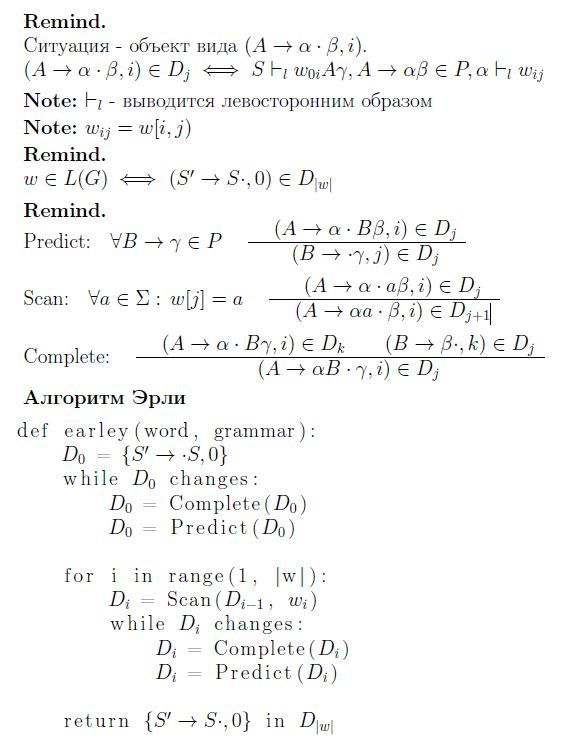
\includegraphics[width=0.75\linewidth]{formal18.JPG}
\end{center}

\newpage

\subsection{22. Алгоритм Эрли синтаксического разбора для КС-грамматик: доказательство корректности.}

Нужно доказать, что алгоритм правильно строит множества $D_0, \dots, D_{|w|}$. Это равносильно тому, что он  поддерживает инвариант вида $(A \rightarrow \alpha \cdot \beta, i) \in D_j \Leftrightarrow \exists \delta \in (\Sigma \cup N)^* ((S \vdash w_{0i} A\delta) \wedge \alpha \vdash w_{ij})$.

\Proof 
$\Rightarrow$. Индукция по построению множеств $D_j$. $(A \rightarrow \alpha \cdot \beta, i)$ попадает в $D_j$ в результате некоторой операции: база - $(S \rightarrow S', 0)$ удовлетворяет инварианту; 

Если операция \textbf{Scan}, то $\alpha = \alpha' a$, $a = w[j - 1]$ и $(A \rightarrow \alpha' \cdot a \beta, i) \in D_{j-1}$. По индукции $S \vdash w_{0i}A\delta$, а значит $\alpha' \vdash w_{i(j - 1)}$. Тогда из равенства $a = w[j - 1]$ следует $\alpha = \alpha' a \vdash  w_{i(j - 1)}w[j - 1] = w_{ij}$. Чтд.

Если операция \textbf{Predict}, то $\alpha = \varepsilon$, $i = j$ - отсюда второй пункт утверждения. Также $\exists i' \leqslant i$ и ситуация $(A' \rightarrow \alpha'A \delta', i') \in D_i$, откуда по индукции $S \vdash w_{0i'}A'\delta'', \alpha' \vdash w_{i'i}. $ Получаем $S \vdash  w_{0i'}A'\delta'' \vdash w_{0i'}\alpha' A \delta' \delta'' \vdash w_{0i'}w_{i'i}A\delta' \delta'' = w_{0i}A \delta$. Чтд.

Если операция \textbf{Complete}, то $\alpha = \alpha' A'$ и $\exists i', \delta$ : $(A \rightarrow \alpha' \cdot A' \beta, i) \in D_{i'}$, $(A' \rightarrow \gamma \cdot, i') \in D_j$. Отсюда $\alpha = \alpha' A' \vdash w_{ii'}w_{i'j} = w_{ij}$; $S \vdash w_{0i}A\delta$ по предположению индукции. Чтд.

$\Leftarrow$. Доказательство индукцией по суммарной длине $w_{0i}A\delta$ из S и $w_{ij}$ из $\alpha$. 

Разбираем случаи в зависимости от $\alpha$. Если $\alpha = \alpha' a$, то $a = w[j-1]$, $\alpha' \vdash w_{i(j-1)}$. По предположению индукции $(A \rightarrow \alpha ' \cdot \beta, i) \in D_{j - 1}$. Тогда по правилу \textit{Scan} получаем  $(A \rightarrow \alpha ' \cdot \beta, i) \in D_{j}$

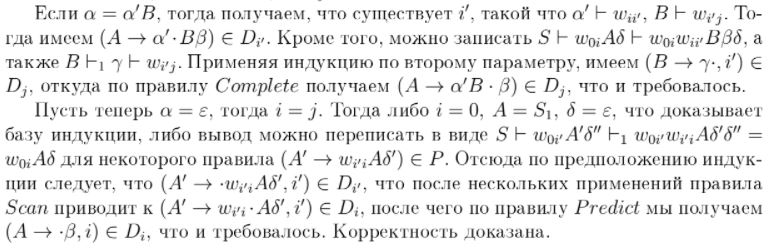
\includegraphics[]{images/formal18_2.JPG}
\EndProof
\newpage{}

\subsection{23. Алгоритм Эрли синтаксического разбора для КС-грамматик: доказательство полноты.}

\Statement Алгоритм Эрли является полным.

\Proof Рассмотрим слово $w$. Если слово $w$ выводимо в грамматике $G = \langle N, \Sigma, P, S \rangle$, то верно, что $S \vdash w$. Пусть $i = 0$, $j = |w|$. Тогда существуют $\varphi, \psi \in \brackets{N \cup \Sigma}^*$, что $\varphi \vdash w[0 : 0] = \varepsilon$, $S \vdash w[0 : |w|] = w$, что $S' \vdash \varphi S' \psi \vdash S' \psi \vdash_1 S \psi$. Укажем явно $\varphi$ и $\psi$: $\varphi = \varepsilon$, $\psi = \varepsilon$, тогда выполняется, что:

\begin{center}
    $S' \vdash_1 S \vdash w$
\end{center}

По сути, только что расписали подробно $S' \vdash w$. $A$ соответствует нетерминальному символу $S'$ (вспомогательному стартовому нетерминалу), $\alpha$ соответствует нетерминальному символу $S$, из которого выводится слово $w$, $\beta$ соответствует пустому слову $\varepsilon$. По основной лемме об инварианте, доказанной ранее, ситуация $\brackets{S' \rightarrow S \cdot, 0} \in D_{|w|}$ тогда и только тогда, когда $S' \vdash w$. Так как из основной леммы следует корректность алгоритма Эрли, то все возможные ситуации будут рассмотрены, и если слово $w$ выводимо в грамматике $G$, то это эквивалентно тому, что будет рассмотрена ситуация $\brackets{S' \rightarrow S \cdot, 0} \in D_{|w|}$, и будет выведено, что $w \in L \brackets{G}$. Если слово $w$ не является выводимым в грамматике $G$, то ситуация $\brackets{S' \rightarrow S \cdot, 0} \notin D_{|w|}$, и будет выведено, что $w \notin L \brackets{G}$. Значит, алгоритм Эрли является полным. \EndProof
\newpage{}

\subsection{24. Алгоритм Эрли синтаксического разбора для КС-грамматик: обоснование сложности. Примеры случаев, где Эрли ведёт себя квадратично. Как реализовать алгоритм Эрли, чтобы он был эффективным}

\textbf{Эффективное хранение ситуаций и правил}

Требуется эффективным образом хранить ситуации типа $\{A \rightarrow \alpha \cdot X \beta, i\} \in D_j$. Множества $D_j$ можно хранить в массиве $D[j][X]$, где $D[j][X] = \{(A_1 \rightarrow \alpha_1 \cdot X \beta_1, i_1), (A_2 \rightarrow \alpha_2 \cdot X \beta_2, i_2), \dots \}$. Возможны три случая, связанные с символом $X$:

\begin{enumerate}
    \item $X = a$, $a \in \Sigma$
    
    \item $X = B$, $B \in N$
    
    \item $X = \$$, $\$$ — конец слова
\end{enumerate}

Правила будем хранить в массиве $G[A]$, где в $G[A]$ будут храниться все правила начинающиеся с $A$, то есть правила вида $A \rightarrow \beta$.

\textbf{Об операциях}

Пусть $w$ — слово.
\begin{enumerate}
\item Scan. $\forall j < |w|:$ $w[j] = a$. Тогда нужно рассмотреть все элементы $D[j][a]$ и расположить их в $D[j + 1]$ в соответствии с символом, следующим за $a$. Асимптотика этой операции соответствует $\mathcal{O} (D[j][a])$, то есть она растёт в соответствии с количеством элементов, находящихся в $D[j][a]$.

\item Predict. $\forall j, B:$ Пусть ситуация имеет вид $(A \rightarrow \alpha \cdot B \beta, i) \in D_j$. Она лежит в $D[j][B]$. Нужно рассмотреть все правила вида $B \rightarrow \gamma \in P$, они лежат в $G[B]$. Асимптотика этой операции $O(D[j][B] \cdot G[B])$.

\item Complete. $\forall j, B:$ Пусть ситуация имеет вид $(B \rightarrow \gamma \cdot, i) \in D_j$, она лежит в $D[j][\$]$. Нужно рассмотреть все ситуации вида $(A \rightarrow \alpha \cdot B \beta, k) \in D_i$, они лежат в $D[i][B]$. Асимптотика этой операции $O(\sum_{i \leq j} G[B] \cdot D[i][B])$.
\end{enumerate}

\textbf{Оценки}

Оценим, как растёт величина $|D_j|$. $D_j = \{(A_1 \rightarrow \alpha_1 . \beta_1, i_1), (A_2 \rightarrow \alpha_2 . \beta_2, i_2), \dots \}$. Пусть $|G|$ — сумма всех длин правых частей правил. Значение $i$ может быть от $0$ до $j$, а точка может быть расположена в $\mathcal{O} (|G|)$ мест, поэтому $\mathcal{O} (|D_j|) = (j + 1)|G|$. 

Асимптотика операции Scan соответствует $\mathcal{O} (|D_j|) = \mathcal{O} (|w| \cdot |G|)$.\\
Асимптотика всех операций Scan $\mathcal{O} (|D_j| \cdot |w|) = \mathcal{O} (|w|^2 \cdot |G|)$.

Для оценки асимптотики операции Predict рассмотрим множества вида:

\begin{center}
    $(A \rightarrow \alpha \cdot B \beta, i) \in D_j$
    
    $(B \rightarrow \cdot \gamma, j) \in D_j$
\end{center}

Так как операция Predict сводится к перебору по $i$, точке и правилам левая часть которых $B$, то асимптотика операции соответствует $\mathcal{O} (D[j][B] \cdot G[B]) = \mathcal{O} (|w| \cdot |G| \cdot G[B])$.

Асимптотика всех операций Predict $O( \sum_{j, B} D[j][B] \cdot G[B] ) = O( |P| \cdot |G| \cdot |w|^2 )$, где $P$ - множество всех правил. 

Рассмотрим теперь операцию Complete. Ситуации из $D[j][\$]$ указывают на номер множества $i$ и нетерминальный символ $B$, который соответствует левой части правила из ситуации. Поэтому для каждой ситуации из $D[j][\$]$ будут рассмотрены все ситуации из $D[i][B]$. Поэтому асимптотика всех операций Complete равна $O(\sum_{j, i \leq j, B} G[B] \cdot D[i][B]) = O(\sum_{j, i \leq j, B} G[B] \cdot D_i) = O(\sum_{j, i \leq j} |P| \cdot D_i) = \mathcal{O} (|P| \cdot |w|^2 \cdot |w| \cdot |G|) = \mathcal{O} ({|w|}^3 {|G|}^2)$.

Так как итераций $\mathcal{O} (|w|)$, то итоговая сложность алгоритма составляет $\mathcal{O} ({|w|}^3{|G|}^2)$. Однако данную оценку можно сильно улучшить, если грамматически удастся доказать (на лекции не стали доказывать), что количество появлений каждого правила ограничена сверху некоторой константой $C$, то асимптотика уже будет равна $\mathcal{O} ({|w|}^2 \cdot C)$. Считаем $|P|, |G|, C$, константами, потому что "вся эта история происходит на стадии компиляции". (в алгоритме мы работаем с одним набором правил, видимо поэтому эти величины можно считать константой)

Есть теорема, что если грамматика однозначна, то алгоритм Эрли для неё стоит квадрат.
Идея доказательства в том, что если грамматика однозначна, то в complete в $(A \rightarrow \alpha \cdot B \beta, k) \in D_i, (B \rightarrow \cdot \gamma, i) \in D_j$ не нужно будет перебирать $i$. Оно будет подбираться однозначно.

Алгоритм за куб.

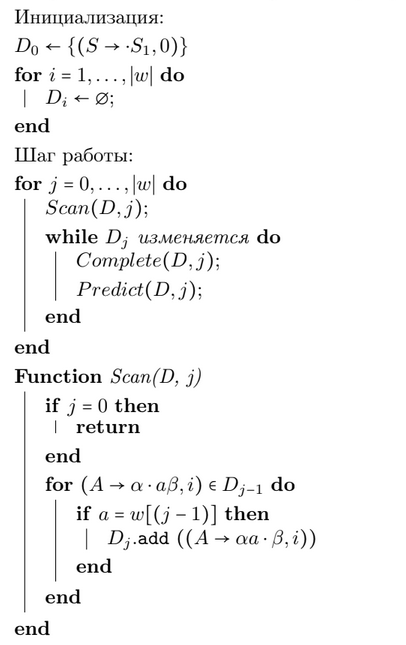
\includegraphics[width=0.45\linewidth]{24_1.png}

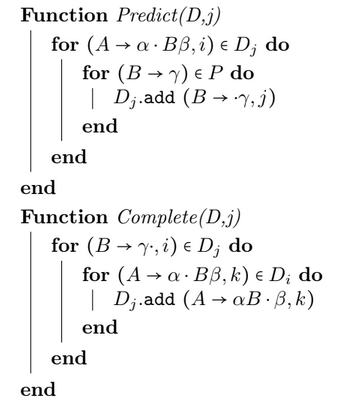
\includegraphics[width=0.4\linewidth]{24_2.png}

Эффективный алгоритм и примеры случаев, где Эрли ведёт себя квадратично: (из neerc.ifmo)

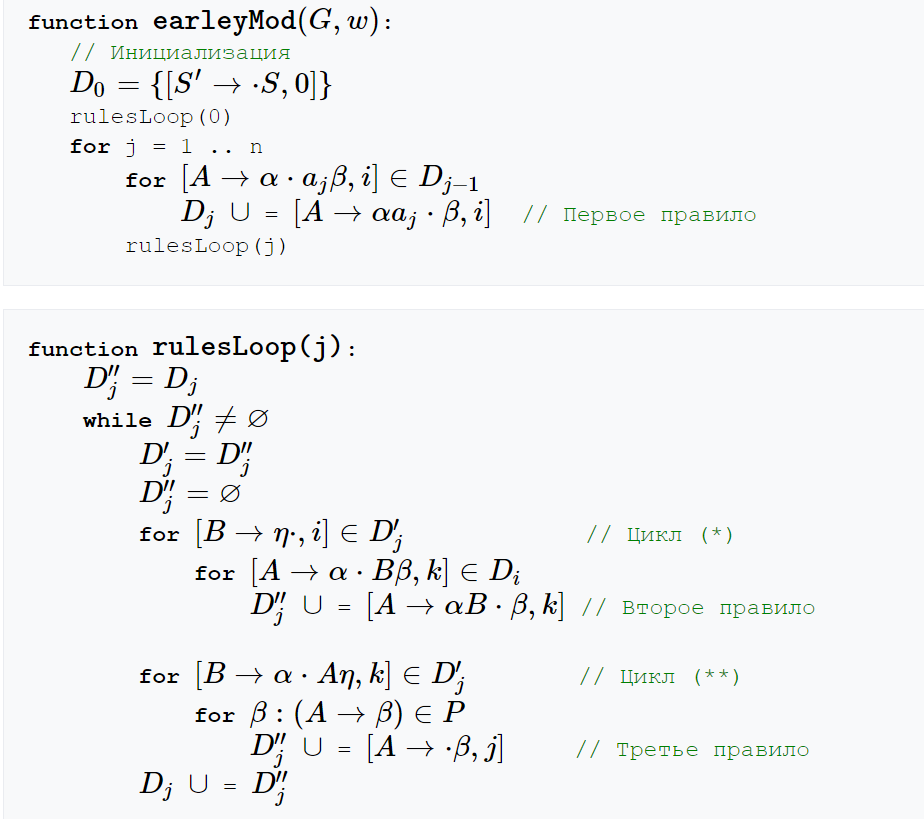
\includegraphics[width=0.8\linewidth]{24_3.png}

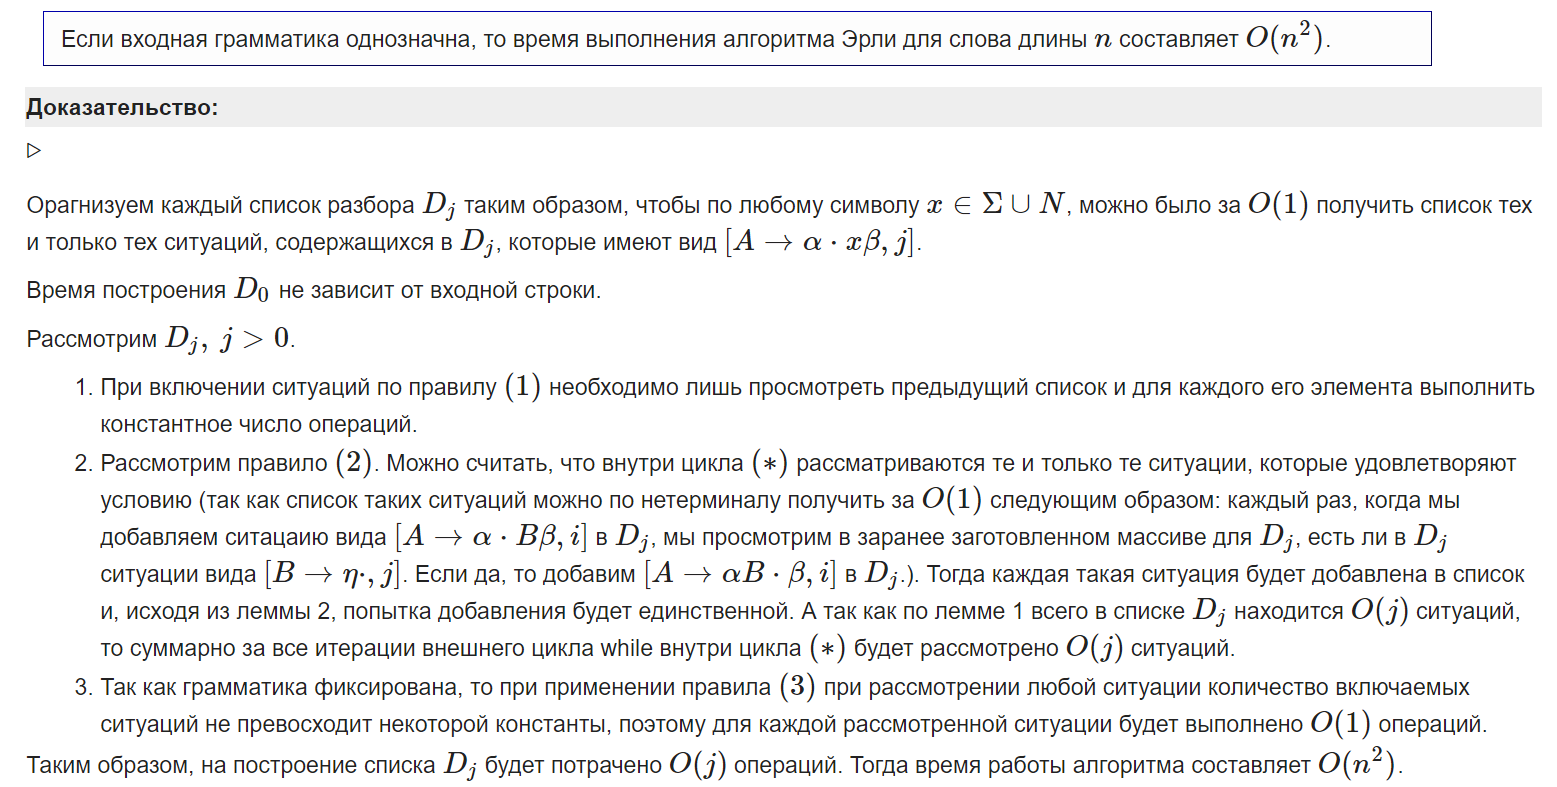
\includegraphics[width=1\linewidth]{24_4.png}
\newpage{}

\Th Пусть для данных $n, k, s$ l: 
\[ C_n^l \cdot \frac{C_{C_n^k - C_{n-l}^k}^s}{C_{C_n^k}^{s}} < 1\]
Тогда $\exists M: \tau(M) > l$

\Proof
Рассмотрим случайное $M = \{M_1, \dots, M_s \}$; количество таких совокупностей - ${C_{C_n^k}^{s}}$. Фиксируем $L \subset R_n, |L| = l$. 

$P(L$ является с.о.п. для $M) = \frac{C_{C_n^k - C_{n-l}^k}^s}{C_{C_n^k}^{s}}$

$P(\exists L, |L| = l: L $ явл. с.о.п. для $M) \leqslant C_n^l \cdot \frac{C_{C_n^k - C_{n-l}^k}^s}{C_{C_n^k}^{s}} < 1$ (по усл. теоремы), значит $\exists M:$ у $M$ нет $l$ - элементных с.о.п.
\EndProof

\Cor \Th Пусть $n \to \infty$, $s=s(n), k=k(n) \to \infty, \frac{sk}{n} \to \infty$

Пусть $ln ln (k) = o(ln \frac{sk}{n}), ln^2 \frac{sk}{n} = o(k), k^2 = o(n)$. 

Тогда $\exists n_0 \forall n > n_0 \exists M: \tau(M) \geqslant \frac{n}{k} ln \frac{sk}{n} - \frac{n}{k} ln ln \frac{sk}{n} - \frac{n}{k} ln ln (k) - \frac{3n}{k} \sim \frac{n}{k} ln \frac{sk}{n}$

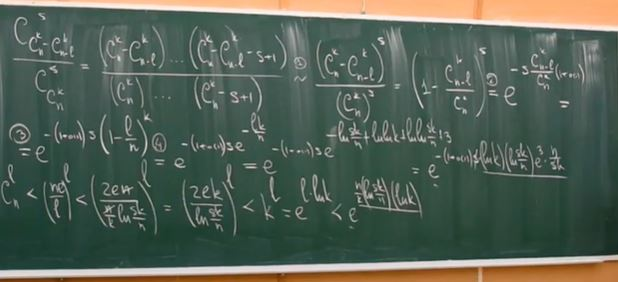
\includegraphics[width=9cm]{images/est4.JPG}

Осталось перемножить е в степенях и понять, что это стремится к нулю, значит, начиная с какого-то $n_0$ оно будет меньше 1.

Проверим переходы:

1) - тут на самом деле верхняя оценка и её достаточно. Ура.

2) - 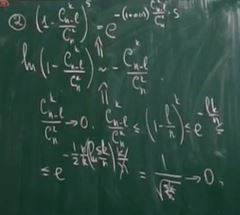
\includegraphics[width=5cm]{images/est6.JPG}

3) - тут надо в ориниальном переходе в правой части поставить $\leqslant$ и вместо $(1 - \frac{l}{n})^k$ написать $(1 - \frac{l}{n-k})^k$.

4) - 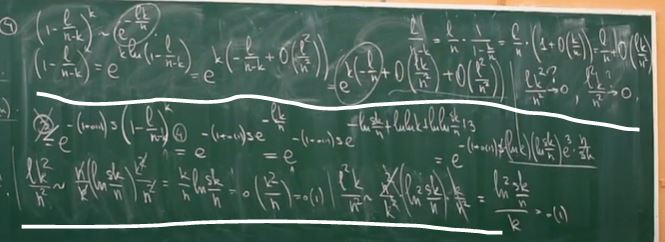
\includegraphics[width=9cm]{images/est7.JPG}
\newpage{}

\subsection{26. Определение LR-грамматики, примеры LR и не LR-грамматик. Стековая аналогия определения (нет конфликтов).  Вопрос на отл: однозначность lr грамматики.}

\Def Грамматика называется LR(k) грамматикой, если LR-k таблица для этой грамматики строится корректно

\Def Для $\alpha \in (N \cup \Sigma)^*$ определим First($\alpha$) как:

First($\alpha$) = $\{a | \alpha\ \rightarrow  au, u \in \Sigma^*\} \cup \{\$\}I(\alpha \rightarrow \varepsilon$)
First($\alpha$) - первый символ, который может вывестись из $\alpha$.

Если $\alpha = a\gamma$, то First($\alpha$) = a

Если $\alpha$ = B$\gamma$, B $\rightarrow \varepsilon$, то First($\alpha$) = First(B) $\cup$ First($\gamma$)
\\
\\
\Def Грамматика называется LR(k) грамматикой, если из условий:
\begin{itemize}
    \item [1.] $S' \rightarrow \cdot \alpha A w \rightarrow \alpha \beta w$
    \item [2.] $S' \rightarrow \cdot \gamma B x \rightarrow \alpha \beta y $ где $\gamma$ - префикс $\alpha$, возможно, несобственный. x - суффикс $w$
    \item [3.] $First_k(w) = First_k(y)$
\end{itemize}
Что происходит в теминах алгоритма? На стеке сейчас лежат $\alpha \beta$ и мы смотрим, верно ли, что можно свернуть однозначно? Наличие двух одинаковых выводов говорит, что нет. То есть алгоритм стоит перед некоторой дилеммой. Можно свернуть А (по правилу $A \rightarrow \beta$) или прочитать что-то еще, и свернуть В(по правилу $B \rightarrow \nu_1 \beta \nu_2$). В первлм случае мы сворачиваем за один шаг, во втором случае - что-то еще сворачиваем, а уже после сворачиваем В.


Что делать в таких ситуациях? А ничего. мы говорим, что такого не допускаем :)


То есть мы говорим, что $\alpha A y = \gamma B x$, то есть $\alpha = \gamma, A = B$
\textbf{Конец определения} \\ \\
\textbf{Примеры LR грамматик}
\begin{itemize}
    \item Грамматика из примера к предыдущему билету
     \item 
     \begin{itemize}
         \item $S \rightarrow A$
         \item $A \rightarrow aA \; | \; b$
     \end{itemize}
     \begin{itemize}
        \item $S \rightarrow A \; | \; aB$
        \item $A \rightarrow aA \; | \; r$
        \item $B \rightarrow aB \; | \; m$
    \end{itemize}
\end{itemize}

Эти грамматики парсятся LR(0), и, соответственно, любой другой грамматикой

\textbf{Любая неоднозначная грамматика - не LR грамматика}
\\
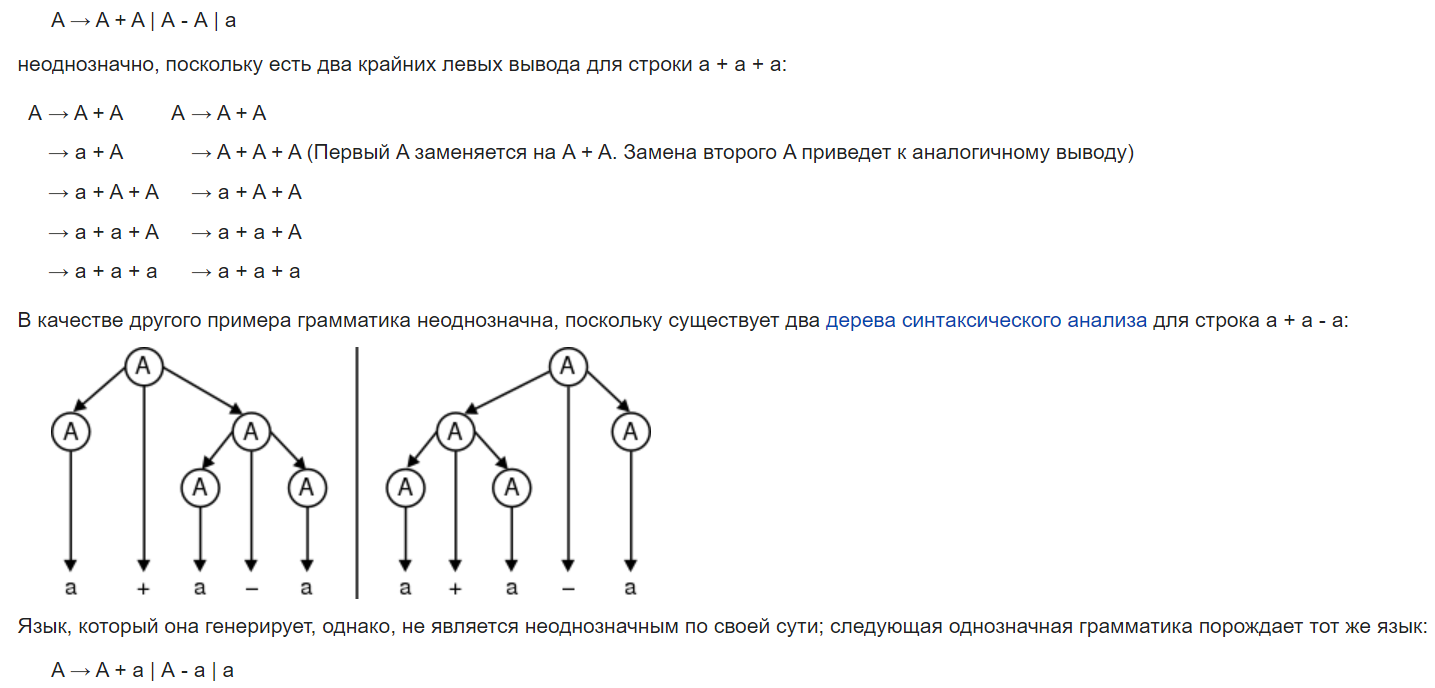
\includegraphics[width=17cm]{formal2.PNG}
\\
\textbf{Дополнительно. Пример грамматики LR(1), не являющейся LR(0) грамматикой}
\begin{itemize}
    \item $S' \rightarrow S$
    \item $S \rightarrow Bb$
    \item $S \rightarrow Cc$
    \item $B \rightarrow a$
     \item $C \rightarrow a$
\end{itemize}
LR(0) разбор
\begin{itemize}
    \item [0] \begin{itemize}
        \item $S' \rightarrow \cdot S$
    \item $S \rightarrow \cdot Bb$
    \item $S \rightarrow \cdot Cc$
    \item $B \rightarrow \cdot a$
     \item $C \rightarrow \cdot a$
    \end{itemize}
    \item [1] \begin{itemize}
        \item $B \rightarrow  a \cdot$
        \item $C \rightarrow a\cdot$
    \end{itemize}
    И все, есть два reduce. Мы не знаем, что делать. А в терминах вывода это означает, что мы могли открыть букву как  ab и как ac, и неважно, что слова разные, у нас уже конфликт в явном виде
\end{itemize}
LR(1) разбор
\begin{itemize}
        \item [0] \begin{itemize}
        \item $S' \rightarrow \cdot S, \$ $
    \item $S \rightarrow \cdot Bb,\$ $
    \item $S \rightarrow \cdot Cc \$$
    \item $B \rightarrow \cdot a, b$
     \item $C \rightarrow \cdot a, c$
    \end{itemize}
    \item [1] \begin{itemize}
        \item $B \rightarrow  a \cdot, b$
        \item $C \rightarrow a\cdot, c$
        \\
        Тут такого противоречия нет, так как мы подсмотрели следующие буквы и поняли, что это соответственно будут reduce(3) и  reduce(4), то есть сейчас мы эти ситуации отличаем
    \end{itemize}
\end{itemize}

\par \textbf{Однозначность LR-грамматики (на отл):}
\begin{figure}[h]
\center{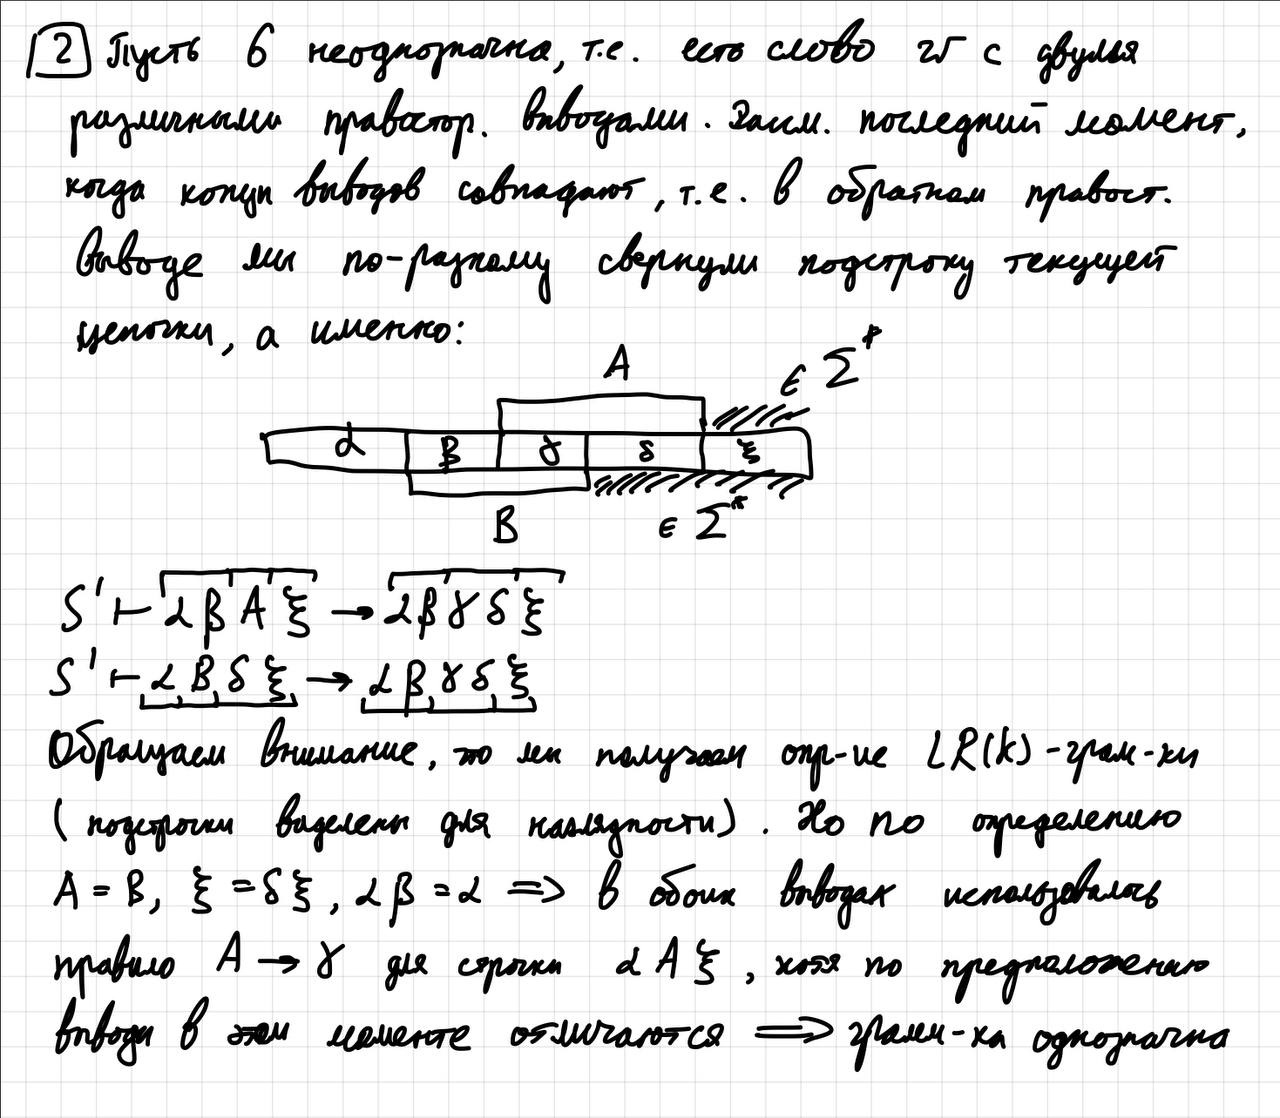
\includegraphics[scale=0.35]{images/LR-unambiguity.jpg}}
\end{figure}
\newpage{}

\subsection{27. Алгоритм построения LR-таблицы. Вопрос на отл: доказательство корректности и полноты. Если верно определение, таблица строится и если не верно, не строится. Критерий LR-овости (отсутствие противоречий).}

\par \Def $A \rightarrow \alpha \cdot \beta, a_1 \ldots a_k$ - LR(k)-ситуация (неформально: если находимся в $A \rightarrow \alpha \cdot \beta$, то $a_1 \ldots a_k$ - первые буквы того, что можем вывести дальше, $a_i \in \Sigma \cup \{\$\}$)
\par \Note Далее будем рассматривать алгоритм LR(1), для $k \neq 1$ действуем аналогично.
\par \Def Пусть $I$ - множество ситуаций. Тогда $CLOSURE(I):=J, I \subset J$, такое что
$$\left.\begin{array}{c}
B \rightarrow \gamma \in P\\
A \rightarrow \alpha_1 \cdot B \alpha_2, a \in J\\
\end{array}
\right\} \Rightarrow \forall c \in First(\alpha_2 a): \: B \rightarrow \cdot \gamma, c \in J$$
\par \Def Пусть $I$ - множество ситуаций, $\lambda \in \Sigma \cup N$. Тогда $$GOTO(I, \lambda):=CLOSURE(\{\langle A \rightarrow \alpha_1 \lambda \cdot \alpha_2 \rangle \: | \: \langle A \rightarrow \alpha_1  \cdot\lambda \alpha_2 \rangle \in I\})$$
\begin{figure}[h]
\center{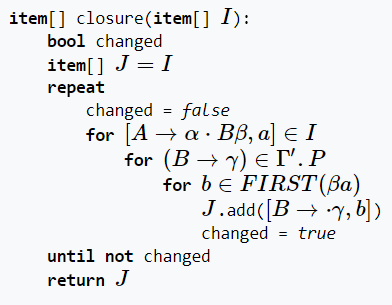
\includegraphics[scale=1]{images/LR(1)-closure.png}
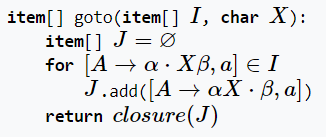
\includegraphics[scale=1]{images/LR(1)-goto.png}}
\end{figure}

\par Построим ДКА, вершинами которого будут множества ситуаций, а на ребрах будут написаны символы из $\Sigma \cup N$, по которым будем делать $GOTO$. Как строим: в начальное состояние добавляем $S' \rightarrow \cdot S, \$$. Затем берем $CLOSURE$ от состояния, делаем $GOTO$ по всем возможным буквам - получаем новые вершины автомата, в которые ведут ребра по этим буквам. Повторяем процесс для добавленных состояний и тд.
\begin{figure}[h]
\center{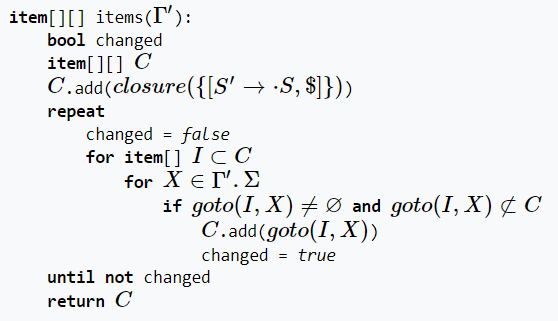
\includegraphics[scale=1]{images/LR(1)-automaton.png}}
\end{figure}
\\
\\
\\
\\
\\
\\
\\
\\


\par Теперь нам остается только построить таблицу $table$ по автомату (столбцы - символы из $N \cup \Sigma \cup \{\$\}$, строки - номера состояний в автомате):
\begin{enumerate}
    \item Если из состояния $i$ в состояние $j$ ведет ребро по букве $a$, то $table[i][a]=(shift, j)$.
    \item Если в состоянии $i$ есть ситуация $A \rightarrow \alpha \cdot, a$, то $table[i][a]=(reduce, j)$, где $j$ - номер правила $A \rightarrow \alpha$ в грамматике. Если нужно записать $(reduce, 0)$, то есть свертка по правилу $S' \rightarrow S$, то записываем $table[i][a]=accept$
    \item Если никакой из прошлых пунктов не записался, то $table[i][a]=error$
\end{enumerate}
\begin{figure}[h]
\center{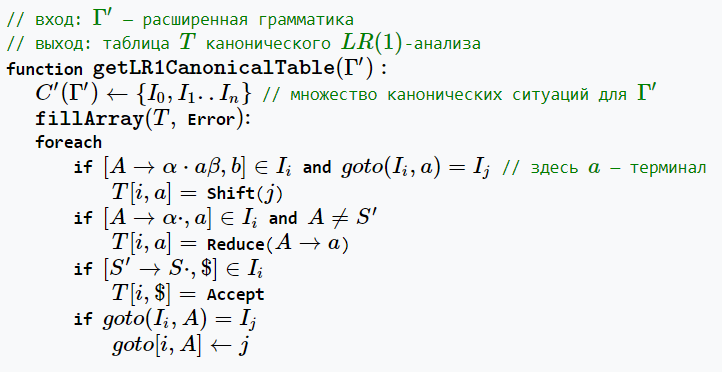
\includegraphics[scale=1]{images/LR(1)-table.png}}
\end{figure}
\newpage{}

\subsection{28. Алгоритм разбора по LR-таблице. Структура стека. Корректность и полнота разбора (на отл).}
\par Пусть у нас есть готовая LR-таблица table и дано слово $w=w_1 \ldots w_n\$$. Создаем стек: изначально записываем в него 0 - номер правила $S' \rightarrow S$, так как оно всегда первое в нашем выводе. Дальше запускаем цикл \begin{enumerate}
    \item Если последний символ на стеке - это номер правила ($i$), то пытаемся дописать на стек следующую букву слова $w_j$: проверяем, если в ячейке $[i, w_j]$ стоит пометка $shift$ (то есть из текущего состояния есть переход по этой букве), то дописываем эту букву на стек, иначе говорим, что слово не лежит в языке.
    \item Берем последние 2 символа со стека: среди них гарантированно одна буква ($c$) и одно число ($k$). Смотрим в ячейку $[k, c]$ \begin{enumerate}
        \item Если там стоит $(shift, to)$, то дописываем на стек $to$ - номер состояния в который надо перейти
        \item Если там стоит $(reduce, rule)$, то находим правило под номером $rule$, удаляем со стека $2 \cdot |rule.right|$ символов (нужно удалить все буквы из этого правила, но на стеке они чередуются с цифрами, поэтому умножаем длину на 2)  и дописать $rule.left$. Если делаем свертку по 0 правилу $S' \rightarrow S$, то есть в этой ячейке стоит Accept, то говорим, что слово лежит в языке.
        \item Если там стоит Error, то слово не лежит в языке
    \end{enumerate}
\end{enumerate}
\par Из алгоритма видно, что на стеке чередуются буквы и числа (в самом начале число)
\newpage{}